\documentclass{article}
\usepackage[utf8]{inputenc}

\title{ET586 - Estatística e Probabilidade Para Computação}
\author{Henrique de Oliveira Braga Sakane}
\date{Abril 2019}

\usepackage{natbib}
\usepackage{graphicx}

\begin{document}

\maketitle

\section{Introdução}
    
 
A disciplina de Estatística e Probabilidade Para Computação tem como foco principal o estudo e analise de gráficos e tabelas, ela utiliza de conceitos estudados em semestres anteriores dos cursos de Ciência e Engenharia da Computação da UFPE para desenvolver conteúdos como: Espaço amostral, probabilidade, medidas, analise exploratória entre outros.
Essa disciplina é oferecida para alunos do 2º período de C.C. e 4º período de E.C. na UFPE e as aulas são ministradas pelas professoras: Renata Souza em C.C. e Marcilia Andrade em E.C.

\section{Relevância}
A cadeira de Estatística e Probabilidade Para Computação é disciplina obrigatória e de grande importância para os alunos de informática, pois praticamente tudo o que acontece no mundo é passível de ser contado, comparado e analisado de alguma forma matemática. O ponto positivo é que a cadeira estimula os alunos a abrir a sua visão de mundo, no que se refere a transformar informações em dados, tornando o aluno capaz de refletir e comparar elementos estatísticos. O ponto negativo visto por alguns alunos é o fato de que há uma demora para relacionar os assuntos de estatística a computação. A disciplina é preenchida com um projeto, essencial para o desenvolvimento das pesquisas relacionadas a areá, ele é o passo final para deixar claro a interação entre problemas computacionais e a estatística.
\begin{table}[hbt!]
\begin{tabular}{|l|l|}
\hline
\multicolumn{1}{|c|}{Disciplina}                                                 & \multicolumn{1}{c|}{Relação}                                                                                                                          \\ \hline
\begin{tabular}[c]{@{}l@{}}MA026- Cálculo diferencial\\  Integral 1\end{tabular} & \begin{tabular}[c]{@{}l@{}}É relacionada a areá de analise, coleta\\ e interpretação de informações.\end{tabular}                                     \\ \hline
\begin{tabular}[c]{@{}l@{}}ET317- Probabilidade e\\  Estatística\end{tabular}    & \begin{tabular}[c]{@{}l@{}}É equivalente em relação a área de estudo:\\ Estatística Descrita; Probabilidade; \\ Estatística Inferencial.\end{tabular} \\ \hline
\end{tabular}
\end{table}

\begin{figure}[hbt!]
\centering
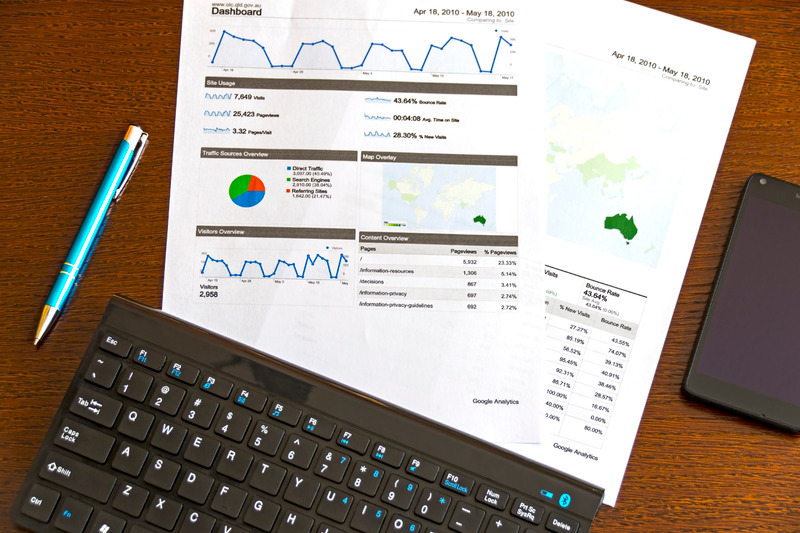
\includegraphics[scale=0.3]{hobs}
\caption{Analise de dados | Licença: Domínio Público  | Fonte: 
https://www.canva.com/photos/business-finance/MADGyemdGh4-blue-click-pen-near-white-document-papers-on-top-of-brown-wooden-table/?query=business}
\label{fig:hobs}
\end{figure}


\bibliographystyle{alpha}
\bibliography{hobs}
\cite{SiteDaDisciplinaCC}
\cite{SiteDaDisciplinaEC}
\cite{ManualDeSobrevivenciaPet}
\cite{PerfilCurricularCC}
\end{document}
